\section{Graph Analysis} \label{graphanalysis}
We created a Jupyter notebook to analyze the graph generated by pydgraph
script. We executed this notebook on the graph generated by one of our
installations which had about 197 packages installed. Below section
explains the results of this analysis.

\subsection{Graph encoding indirect dependencies} \label{graphvariation}
The graph created by pydgraph script captures the direct relationship between
the nodes. This essentially means than if package A depends on package B then
 there will be edge between node A and node B. However, if package C depends
 on package B, then indirectly, it also depends on package A. In the graph
 created by pydgraph, the edge between A and C is not created.
 We created another variation of the graph(called GNew) which adds a link for
  such indirect dependencies. So, in GNew, an edge between A and C exists.

\subsection{Degree Distribution} \label{degreedist}
The fig ~\ref{fig:gdegree} shows the degree distribution of original graph while
the fig ~\ref{fig:gnewdegree}  shows the degree distribution of the new graph
which has
indirect dependencies encoded.
After observing these graphs, we can say that
 \begin{itemize}
 \item The orignial graph (G) does not seem to follow degree distribution
 pattern of scale free graph. Especially on the log-log scale, it in not a
 straight line like in scale free graph.
 \item However, the updated graph (GNew) where indirect dependencies are
 directly added to each node, the graph looks like scale free graph with
 power law degree distribution
\end{itemize}


\begin{figure}[htbp]
\centering
\fbox{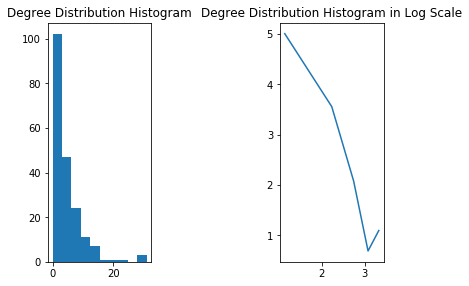
\includegraphics[width=\linewidth]{images/GDegreeDist.png}}
\caption{Degree distribution of original graph}
\label{fig:gdegree}
\end{figure}

\begin{figure}[htbp]
\centering
\fbox{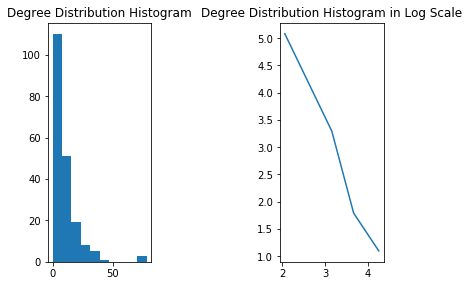
\includegraphics[width=\linewidth]{images/GNewDegreeDist.png}}
\caption{Degree distribution of indirect-dependency-graph}
\label{fig:gnewdegree}
\end{figure}


\subsection{In and Out Degree} \label{inoutdegree}
The analysis of in-degree and out-degree of GNew can explain us the packages
which has large number of dependencies and packages which are used by other
packages a lot.
The higher value of in-degree means the package depends on several other
packages. Similarly, higher value of out-degree means the package is used by
several other packages.
After observing fig ~\ref{fig:indegree} we can say that nodes (packages) like
 "uniq" or "zope.publiser" have larger dependency on other packages.
Fig ~\ref{fig:outdegree} explains that packages like "setuptools", "six" and
 "zope.interface" are used by several other packages.

\begin{figure}[htbp]
\centering
\fbox{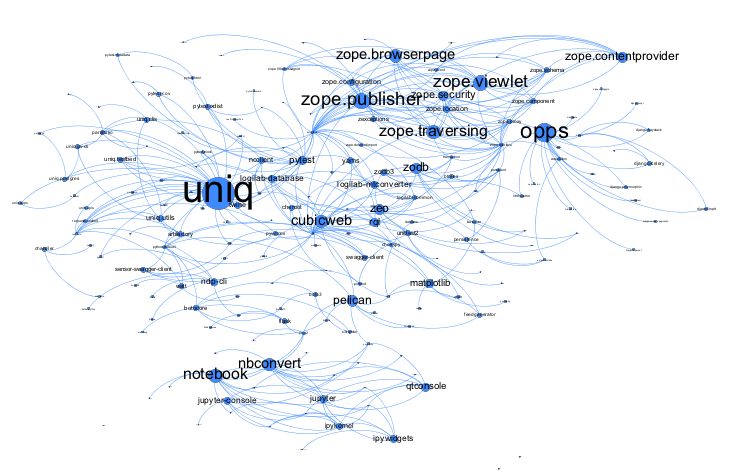
\includegraphics[width=\linewidth]{images/indegree.png}}
\caption{In-Degree of indirect-dependency-graph}
\label{fig:indegree}
\end{figure}

\begin{figure}[htbp]
\centering
\fbox{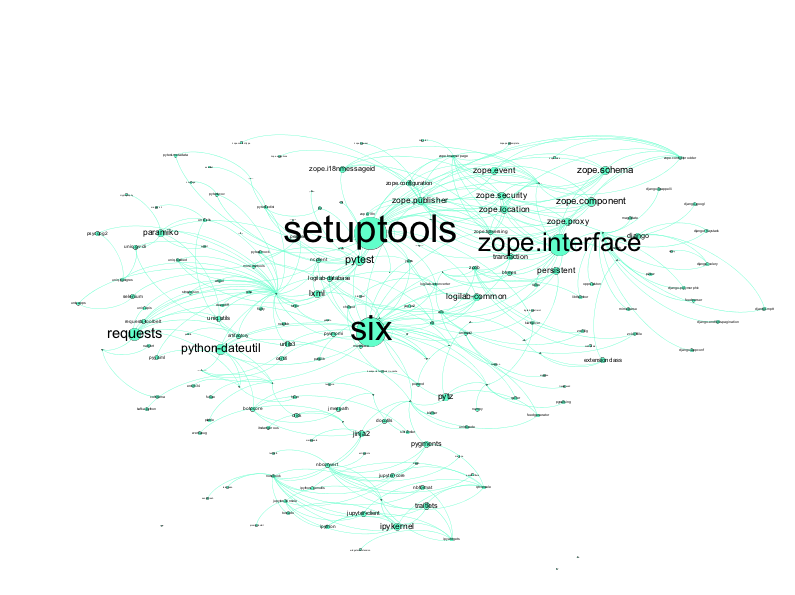
\includegraphics[width=\linewidth]{images/outdegree.png}}
\caption{Out-Degree of indirect-dependency-graph}
\label{fig:outdegree}
\end{figure}


\subsection{Friendship Paradox} \label{friend}
For original graph, only 21 percent nodes follow friendship paradox. However,
 for
indirect-dependency-graph, the firendship paradox holds true for about 83
percent
nodes.This is very useful since using indirect dependency graph, we can
quickly identify the hubs in this network. Essentially, we can identify the
popular packages very easily without even knowing degree distributio of
entire network.

\subsection{Communities} \label{comm}
Fig ~\ref{fig:community} explains that the network has large number of
communities. In this specific installation, it can be observed that:
 \begin{itemize}
\item There are 10 identified communities (used resolution factor of 5). The
bigger communities can be easily explained. For example, community around
testing packages like pytest, community around notebook packages (notebook,
nbconvert, ipykernel), communiy around django and community arond zope.
\item This installation has bunch of completely separate packages like 1) pip
and pipdeptree 2)flake and 3)networkx and decorator
\item The node size indicates betweenness centrality. It looks like pytest is
the one which is used mostly across all communities.
\end{itemize}
\begin{figure}[htbp]
\centering
\fbox{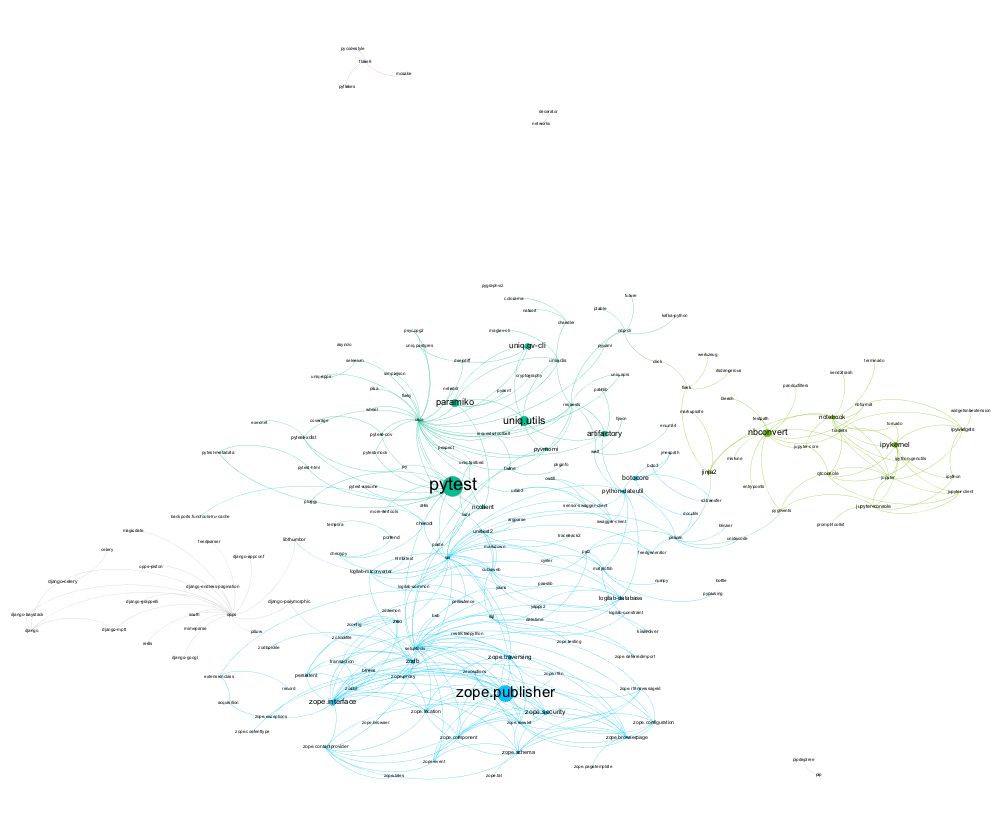
\includegraphics[width=\linewidth]{images/communities.png}}
\caption{Communities}
\label{fig:community}
\end{figure}


\subsection{Change Propogation} \label{change}
This network can also be utilized for several other purposes. For example, if
 package A is undergoing a major release, we can identify all the dependent
 packages to understand the impact of the change. The paths between two nodes
  can explain the different ways changes in Package A impacts Package B.
  Fig ~\ref{fig:impact} and Fig ~\ref{fig:impactind}  explains this.

\begin{figure}[htbp]
\centering
\fbox{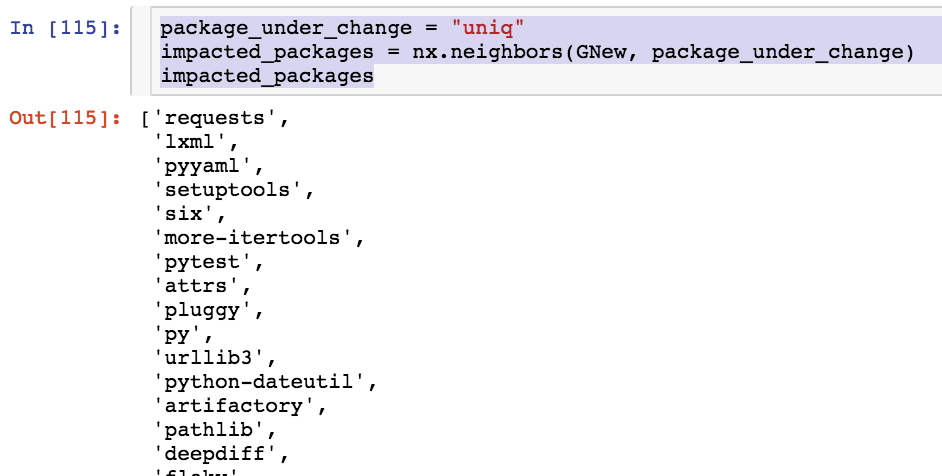
\includegraphics[width=\linewidth]{images/impact.png}}
\caption{Impact of Change}
\label{fig:impact}
\end{figure}

\begin{figure}[htbp]
\centering
\fbox{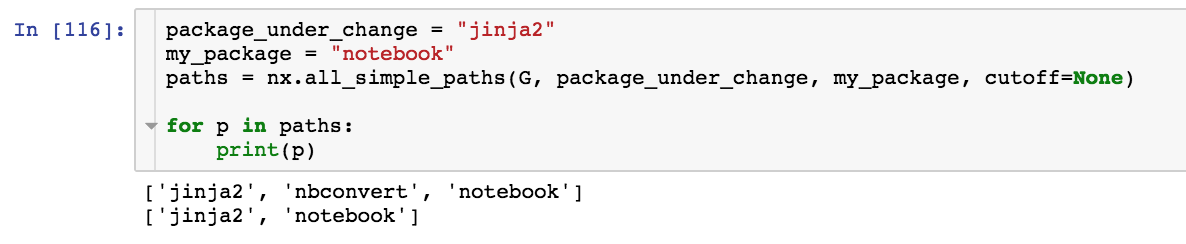
\includegraphics[width=\linewidth]{images/impactind.png}}
\caption{Impact of Change}
\label{fig:impactind}
\end{figure}